\documentclass[]{article}
\usepackage{lmodern}
\usepackage{amssymb,amsmath}
\usepackage{ifxetex,ifluatex}
\usepackage{fixltx2e} % provides \textsubscript
\ifnum 0\ifxetex 1\fi\ifluatex 1\fi=0 % if pdftex
  \usepackage[T1]{fontenc}
  \usepackage[utf8]{inputenc}
\else % if luatex or xelatex
  \ifxetex
    \usepackage{mathspec}
  \else
    \usepackage{fontspec}
  \fi
  \defaultfontfeatures{Ligatures=TeX,Scale=MatchLowercase}
\fi
% use upquote if available, for straight quotes in verbatim environments
\IfFileExists{upquote.sty}{\usepackage{upquote}}{}
% use microtype if available
\IfFileExists{microtype.sty}{%
\usepackage{microtype}
\UseMicrotypeSet[protrusion]{basicmath} % disable protrusion for tt fonts
}{}
\usepackage[margin=1in]{geometry}
\usepackage{hyperref}
\hypersetup{unicode=true,
            pdftitle={Inferring the existence and direction of causal associations in the face of measurement error},
            pdfborder={0 0 0},
            breaklinks=true}
\urlstyle{same}  % don't use monospace font for urls
\usepackage{graphicx,grffile}
\makeatletter
\def\maxwidth{\ifdim\Gin@nat@width>\linewidth\linewidth\else\Gin@nat@width\fi}
\def\maxheight{\ifdim\Gin@nat@height>\textheight\textheight\else\Gin@nat@height\fi}
\makeatother
% Scale images if necessary, so that they will not overflow the page
% margins by default, and it is still possible to overwrite the defaults
% using explicit options in \includegraphics[width, height, ...]{}
\setkeys{Gin}{width=\maxwidth,height=\maxheight,keepaspectratio}
\IfFileExists{parskip.sty}{%
\usepackage{parskip}
}{% else
\setlength{\parindent}{0pt}
\setlength{\parskip}{6pt plus 2pt minus 1pt}
}
\setlength{\emergencystretch}{3em}  % prevent overfull lines
\providecommand{\tightlist}{%
  \setlength{\itemsep}{0pt}\setlength{\parskip}{0pt}}
\setcounter{secnumdepth}{0}
% Redefines (sub)paragraphs to behave more like sections
\ifx\paragraph\undefined\else
\let\oldparagraph\paragraph
\renewcommand{\paragraph}[1]{\oldparagraph{#1}\mbox{}}
\fi
\ifx\subparagraph\undefined\else
\let\oldsubparagraph\subparagraph
\renewcommand{\subparagraph}[1]{\oldsubparagraph{#1}\mbox{}}
\fi

%%% Use protect on footnotes to avoid problems with footnotes in titles
\let\rmarkdownfootnote\footnote%
\def\footnote{\protect\rmarkdownfootnote}

%%% Change title format to be more compact
\usepackage{titling}

% Create subtitle command for use in maketitle
\newcommand{\subtitle}[1]{
  \posttitle{
    \begin{center}\large#1\end{center}
    }
}

\setlength{\droptitle}{-2em}
  \title{Inferring the existence and direction of causal associations in the face
of measurement error}
  \pretitle{\vspace{\droptitle}\centering\huge}
  \posttitle{\par}
  \author{}
  \preauthor{}\postauthor{}
  \predate{\centering\large\emph}
  \postdate{\par}
  \date{19 February 2017}

\begin{document}
\maketitle

Gibran Hemani*, Kate Tilling and George Davey Smith

MRC Integrative Epidemiology Unit (IEU) at the University of Bristol,
School of Social and Community Medicine, Bristol, UK

* Correspondence to:
\href{mailto:g.hemani@bristol.ac.uk}{\nolinkurl{g.hemani@bristol.ac.uk}}

\subsubsection{Abstract}\label{abstract}

Inference of the causal structure that induces correlations between two
traits can be achieved by combining genetic associations with a
mediation-based approach, as is done in the causal inference test (CIT)
and others. However, we show that measurement error in the phenotypes
can lead to mediation-based approaches inferring the wrong causal
direction, and that increasing sample sizes has the adverse effect of
increasing confidence in the wrong answer. Here we introduce an
extension to Mendelian randomisation, a method that uses genetic
associations in an instrumentation framework, that enables inference of
the causal direction between traits, with some advantages. First, it is
less susceptible to bias in the presence of measurement error; second,
it is more statistically efficient; third, it can be performed using
only summary level data from genome-wide association studies; and
fourth, its sensitivity to measurement error can be evaluated. We apply
the method to infer the causal direction between DNA methylation and
gene expression levels. Our results demonstrate that, in general, DNA
methylation is more likely to be the causal factor, but this result is
highly susceptible to bias induced by systematic differences in
measurement error between the platforms. We emphasise that, where
possible, implementing MR and appropriate sensitivity analyses alongside
other approaches such as CIT is important to triangulate reliable
conclusions about causality.

\subsection{Introduction}\label{introduction}

Observational measures of the human phenome are growing ever more
abundant, but using these data to make causal inference is notoriously
susceptible to many pitfalls, with basic regression-based techniques
unable to distinguish a true causal association from reverse causation
or confounding\textsuperscript{1--3}. In response to this, genetic
instrumentation has emerged as a technique for improving the reliability
of causal inference in observational data, and with the coincident rise
in genome-wide association studies it is now a prominent tool that is
applied in several different guises\textsuperscript{3--6}. However,
potential pitfalls remain and one that is often neglected is the
influence of non-differential measurement error on the reliability of
causal inference.

Measurement error is the difference between the measured value of a
quantity and its true value. This study focuses specifically on
non-differential measurement error where all strata of a measured
variable have the same error rate, which can manifest as changes in
scale or levels of imprecision (noise) of the measurement. Such
variability can arise through a whole plethora of mechanisms, which are
often unique to the study design and difficult to
avoid\textsuperscript{7,8}. Array technology is now commonly used to
obtain high throughput phenotyping at low cost, but comes with the
problem of having imperfect resolution, for instance methylation levels
as measured by the Illumina450k chip are prone to have some amount of
noise around the true value due to imperfect
sensitivity\textsuperscript{9,10}. Relatedly, if the measurement of
biological interest is the methylation level in a T cell, then
measurement error of this value can be introduced by using methylation
levels from whole blood samples because the measured value will be an
assay of many cell types\textsuperscript{11}.

Measurement error will of course arise in other types of data too. For
example when measuring BMI one is typically interested in using this as
a proxy for adiposity, but it is clear that the correlation between BMI
and underlying adiposity is not perfect\textsuperscript{12}. A similar
problem of biological misspecification is unavoidable in disease
diagnosis, and measuring behaviour such as smoking or diet is
notoriously difficult to do accurately. Measurement error can also be
introduced after the data has been collected, for example the
transformation of non-normal data for the purpose of statistical
analysis will lead to a new variable that will typically incur both
changes in scale and imprecision (noise) compared to the original
variable. The sources of measurement error are not limited to this
list\textsuperscript{8}, and its impact has been explored in the
epidemiological literature extensively\textsuperscript{13,14}. Given the
near-ubiquitous presence of measurement error in phenomic data it is
vital to understand its impact on the tools we use for causal inference.

An established study design that can provide information about causality
is randomisation. Given the hypothesis that trait A (henceforth referred
to as the exposure) is causally related to trait B (henceforth referred
to as the outcome), randomisation can be employed to assess the causal
nature of the association by randomly splitting the sample into two
groups, subjecting one group to the exposure and treating the other as a
control. The association between the exposure and the outcome in this
setting provides a robust estimate of the causal relationship. This
provides the theoretical basis behind randomised control trials, but in
practice randomisation is often impossible to implement in an
experimental context due to cost, scale or inability to manipulate the
exposure. The principle, however, can be employed in extant
observational data through the use of genetic variants associated with
the exposure (instruments), where the inheritance of an allele serves as
a random lifetime allocation of differential exposure
levels\textsuperscript{15,16}. Two statistical approaches to exploiting
the properties of genetic instruments are widely used: mediation-based
approaches and Mendelian randomisation (MR).

Mediation-based approaches employ genetic instruments (typically single
nucleotide polymorphisms, SNPs) to orient the causal direction between
the exposure and the outcome. If a SNP is associated with an exposure,
and the exposure is associated with some outcome, then it logically
follows that the indirect influence of the SNP on the outcome will
disappear when conditioning on the exposure. Here, the exposure
`mediates' the association between the SNP and the outcome, providing
information about the causal influence of the exposure on the outcome.
This forms the basis of a number of methods such as genetical
genomics\textsuperscript{17}, the regression-based causal inference test
(CIT)\textsuperscript{4,18}, a structural equation modelling (SEM)
implementation in the NEO software\textsuperscript{5}, and various other
methods including Bayesian approaches\textsuperscript{6}. They have been
employed by a number of recent publications that make causal inferences
in large scale `omics datasets\textsuperscript{6,19--23}.

MR can be applied to the same data - phenotypic measures of the exposure
and the outcome variables and a genetic instrument for the exposure -
but the genetic instrument is employed in a subtly different manner.
Here the SNP is used as a surrogate for the exposure. Assuming the SNP
associates with the outcome only through the exposure, the causal effect
of the exposure on the outcome can be estimated by scaling the
association between the SNP and the outcome by the association between
the SNP and the exposure. Though difficult to test empirically, this
assumption can be relaxed in various ways when multiple instruments are
available for a putative exposure\textsuperscript{24,25} and a number of
sensitivity tests are now available to improve
reliability\textsuperscript{26}.

By utilising genetic instruments in different ways, mediation-based
analysis and MR models have properties that confer some advantages and
some disadvantages for reliable causal inference. In the CIT framework
(described fully in the Methods) for example, the test statistic is
different if you test for the exposure causing the outcome or the
outcome causing the exposure, allowing the researcher to infer the
direction of causality between two variables by performing the test in
both directions and choosing the model with the strongest evidence. The
CIT also has the valuable property of being able to distinguish between
several putative causal graphs that link the traits with the SNP (Figure
1). Such is not the case for MR, where in order to infer the direction
of causality between two traits the instrument must be known to
influence the exposure primarily, associating with the outcome only
through the exposure.

Assuming biological knowledge of genetic associations can be problematic
because if there exists a putative association between two variables,
with the SNP being robustly associated with each, it can be difficult to
determine which of the two variables is subject to the primary effect of
the SNP (i.e.~for which of the two variables is the SNP a valid
instrument? Figure 1). By definition, we expect that if the association
is causal then a SNP for the exposure will be associated with the
outcome, such that if the researcher erroneously uses the SNP as an
instrument for the outcome then they are likely to see an apparently
robust causal association of outcome on exposure. Such a situation can
arise in many scenarios. Genome-wide association studies (GWASs) that
identify genetic associations for complex traits are, by design,
hypothesis free and agnostic of genomic function, and it often takes
years of follow up studies to understand the biological nature of a
putative GWAS hit\textsuperscript{27}. If multiple instruments are
available for an hypothesised exposure, which is increasingly typical
for complex traits that are analysed in large GWAS consortia, then
techniques can be applied to mitigate these issues\textsuperscript{16}.
But these techniques cannot always be applied in the case of determining
causal directions between 'omic measures where typically only one
cis-acting SNP is known. For example if a DNA methylation probe is
associated with expression of an adjacent gene, then is a cis-acting SNP
an instrument for the DNA methylation level, or the gene expression
level (Figure 1)?

MR has some important advantages over the mediation-based approaches.
The mediation-based approaches require that the exposure, outcome and
instrumental variables are all measured in the same data, whereas recent
extensions to MR circumvent this requirement, allowing causal inference
to be drawn when exposure variables and outcome variables are measured
in different samples\textsuperscript{28}. This has the crucial advantage
of improving statistical power by allowing analysis in much larger
sample sizes, and dramatically expands the breadth of possible
phenotypic relationships that can be evaluated\textsuperscript{26}.
Additionally, when MR assumptions are satisfied the method is robust to
there being measurement error in the exposure
variable\textsuperscript{29}. Indeed instrumental variable (IV) analysis
was in part initially introduced as a correction for measurement error
in the exposure\textsuperscript{30}, whereas it has been noted that both
classic mediation-based analyses\textsuperscript{13,14,31,32} and
mediation-based methods that use instrumental
variables\textsuperscript{33,34} are prone to be unreliable in its
presence.

Using theory and simulations we show how non-differential measurement
error in phenotypes can lead to unreliable causal inference in the
mediation-based CIT method. We then present an extension to MR that
allows researchers to ascertain the causal direction of an association
even when the biology of the instruments are not fully understood, and
also a matric to evaluate the sensitivity of the result of this
extension to measurement error. Together these extensions improve the
utility of MR in cases where mediation based methods might have
otherwise been used preferentially. Finally, we apply this new method to
infer the direction of causation between DNA methylation levels and gene
expression levels. Our analyses highlight that because these different
causal inference techniques have varying strengths and weaknesses,
triangulation of evidence from as many sources as possible should be
practiced in causal inference\textsuperscript{35}.

\subsection{Model}\label{model}

We can model a system whereby some exposure \(x\) has a causal influence
\(\beta_x\) on an outcome \(y\) such that

\[
y = \alpha_x + \beta_x x + \epsilon_x
\]

In addition, the exposure is influenced by a SNP \(g\) with an effect of
\(\beta_g\) such that

\[
x = \alpha_g + \beta_g g + \epsilon_g
\]

The \(\alpha_*\) terms represent intercepts, and the \(\epsilon_*\)
denote random error. Mediation-based analyses that test whether \(x\)
causally relates to \(y\) impinge on evaluating if the influence of
\(g\) on \(y\) can be accounted for by conditioning on \(x\), such that

\[
cov(g, y - \hat{y}) = 0
\]

where \(\hat{y} = \hat{\alpha}_x + \hat{\beta}_x x_o\). MR analysis
estimates the causal influence of \(x\) on \(y\) by using the instrument
as a proxy for \(x\), such that

\[
\begin{aligned}
\hat{x} & = \hat{\beta}_g g \\
y & = \beta_{MR}\hat{x} + \epsilon_{MR}
\end{aligned}
\]

where \(\beta_{MR} \neq 0\) denotes the existence of causality, and
\(\beta_{MR}\) is an estimate of the causal effect.

Measurement error of an exposure can be modeled as a transformation of
the true value that leads to the observed value, \(x_o = f(x)\). For
example, following Pierce and VanderWeele\textsuperscript{29} we can
define

\[
f(x) = \alpha_{mx} + \beta_{mx} x + \epsilon_{mx}
\]

where \(\alpha_{mx}\) and \(\beta_{mx}\) influence the error in the
measurement of \(x\) by altering its scale, and \(\epsilon_{mx}\)
represents the imprecision (or noise) in the measurement of \(x\). The
same model of measurement error can be applied to the outcome variable
\(y\). In this study we assume there is no measurement error in the SNP
and measurement error in the exposure and the outcome are uncorrelated.

\subsection{Methods}\label{methods}

\subsubsection{CIT test}\label{cit-test}

The CIT method\textsuperscript{4} is implemented in the R package
\emph{R/cit}\textsuperscript{18}. The methodology of the CIT is as
follows. Assume an exposure \(x\) is instrumented by a SNP \(g\), and
the exposure \(x\) causes an outcome \(y\), as described above. The
following tests are then performed:

\begin{enumerate}
\def\labelenumi{\arabic{enumi}.}
\tightlist
\item
  \(H_0: cov(g, x) = 0; H_1: cov(g, x) \neq 0\); \emph{the SNP
  associates with the exposure}
\item
  \(H_0: cov(g, y) = 0; H_1: cov(g, y) \neq 0\); \emph{the SNP
  associates with the outcome}
\item
  \(H_0: cov(x, y) = 0; H_1: cov(x, y) \neq 0\); \emph{the exposure
  associates with the outcome}
\item
  \(H_0: cov(g, y - \hat{y}) \neq 0; H_1: cov(g, y - \hat{y}) = 0\);
  \emph{the SNP is independent of the outcome when the outcome is
  adjusted for the exposure}
\end{enumerate}

where \(y - \hat{y} = y - \hat{\alpha}_g + \hat{\beta}_g x\) is the
residual of \(y\) after adjusting for \(x\), where \(x\) is assumed to
mediate the association between the SNP and the outcome. If all four
tests reject the null hypothesis then it is inferred that \(x\) causes
\(y\). The CIT measures the strength of causality by generating an
omnibus p-value, \(p_{CIT}\), which is simply the largest (least
extreme) p-value of the four tests, the intuition being that causal
inference is only as strong as the weakest link in the chain of tests.

In these analyses the \emph{cit.cp} function was used to obtain an
omnibus p-value. To infer the direction of causality using the CIT
method, an omnibus p-value generated by CIT, \(p_{CIT}\), was estimated
for the direction of \(x\) causing \(y\) (Model 1), and for the
direction of \(y\) causing \(x\) (Model 2). For some significance
threshold \(\alpha\), the existence of causality and its direction was
inferred based on the following scenarios:

\begin{itemize}
\tightlist
\item
  If \(p_{CIT, x \rightarrow y} < \alpha\) and
  \(p_{CIT, y \rightarrow x} > \alpha\) then model 1 is accepted
\item
  If \(p_{CIT, x \rightarrow y} > \alpha\) and
  \(p_{CIT, y \rightarrow x} < \alpha\) then model 2 is accepted
\item
  If \(p_{CIT, x \rightarrow y} > \alpha\) and
  \(p_{CIT, y \rightarrow x} > \alpha\) then no evidence for a causal
  relationship
\item
  If \(p_{CIT, x \rightarrow y} < \alpha\) and
  \(p_{CIT, y \rightarrow x} < \alpha\) then the confounding model is
  accepted (\(x \leftarrow g \rightarrow y\)).
\end{itemize}

For the purposes of compiling simulation results we use an arbitrary
\(\alpha = 0.05\) value, though we stress that for real analyses it is
not good practice to rely on p-values for making causal inference, nor
is it reliable to depend on arbitrary significance
thresholds\textsuperscript{36}.

\subsubsection{MR causal test}\label{mr-causal-test}

Two stage least squares (2SLS) is a commonly used technique for
performing MR when the exposure, outcome and instrument data are all
available in the same sample. A p-value for this test, \(p_{MR}\), was
obtained using the R package \(R/systemfit\)\textsuperscript{37}.

The method that we will now describe is designed to distinguish between
two models, \(x \rightarrow y\) or \(y \rightarrow x\). Unlike the CIT
framework, this approach cannot infer if the true model is
\(x \leftarrow g \rightarrow y\). We also assume all genetic effects are
additive.

To infer the direction of causality it is desirable to know which of the
variables, \(x\) or \(y\), is being directly influenced by the
instrument \(g\). This can be achieved by assessing which of the two
variables has the biggest absolute correlation with \(g\) (Appendix 2),
formalised by testing for a difference in the correlations \(\rho_{gx}\)
and \(\rho_{gy}\) using Steiger's Z-test for correlated correlations
within a population\textsuperscript{38}. It is calculated as

\[
Z = (Z_{gx} - Z_{gy}) \frac{\sqrt{N-3}}{\sqrt{2(1-\rho_{xy})h}}
\]

where Fisher's z-transformation is used to obtain
\(Z_{g*} = \frac{1}{2} \ln \left ( \frac{1+\rho_{g*}}{1-\rho_{g*}} \right )\),

\[
h = \frac{1 - (frm^2)} {1 - rm^2}
\]

where

\[
f = \frac{1 - \rho_{xy}}{2(1 - rm^2)}
\]

and

\[
rm^2 = \frac{1}{2}(\rho_{gx}^2 + \rho_{gy}^2).
\]

The \(Z\) value is interpreted such that

\[
Z \left\{
\begin{array}{ll}
> 0, & x \to y\\
< 0, & y \to x\\
= 0, & x \perp\!\!\!\perp y 
\end{array} \right.
\]

and a p-value is generated from the \(Z\) value to indicate the
probability of obtaining the observed difference in correlations
\(\rho_{gx}\) and \(\rho_{gy}\) under the null hypothesis that both
correlations are identical. The existence of causality and its direction
is inferred based on the following scenarios:

\begin{itemize}
\tightlist
\item
  If \(p_{Steiger} < \alpha\) and \(p_{MR} < \alpha\) and \(Z > 0\) then
  a causal association for the correct model is accepted
\item
  If \(p_{Steiger} < \alpha\) and \(p_{MR} < \alpha\) and \(Z < 0\) then
  a causal association for the incorrect model is accepted
\item
  Otherwise no evidence for a causal relationship
\end{itemize}

For the purposes of compiling simulation results, we use an arbitrary
\(\alpha = 0.05\) value.

Note that the same correlation test approach can be applied to a
two-sample MR\textsuperscript{28} setting. Two-sample MR refers to the
case where the SNP-exposure association and SNP-outcome association are
calculated in different samples (e.g.~from publicly available summary
statistics). Here the Steiger test of two independent correlations can
be applied where.

\[
Z = \frac{Z_{gx} - Z_{gy}} { \sqrt{ 1 / (N_{1} - 3) + 1 / (N_{2} - 3) } }
\]

An advantage of using the Steiger test in the two sample context is that
it can compare correlations in independent samples where sample sizes
are different. Steiger test statistics were calculated using the
\emph{r.test} function in the R package
\emph{R/psych}\textsuperscript{39}.

\subsubsection{Causal direction sensitivity
analysis}\label{causal-direction-sensitivity-analysis}

The Steiger test for inferring if \(x \rightarrow y\) is based on
evaluating \(\rho_{gx} > \rho_{gy}\). However, \(\rho_{gx}\) and
\(\rho_{gy}\) are underestimated if \(x\) and \(y\) are measured
imprecisely. If, for example, \(x\) has lower measurement precision than
\(y\) then we might empirically obtain \(\rho_{g,x_o} < \rho_{g,y_o}\)
because \(\rho_{g,x_o}\) could be underestimated more than
\(\rho_{g,y_o}\).

As we show in Appendix 2 it is possible to infer the bounds of
measurement error on \(x_o\) or \(y_o\) given known genetic
associations. The maximum measurement error of \(x_o\) is
\(\rho_{g,x_o}\), because it is known that at least that much of the
variance has been explained in \(x_o\) by \(g\). The minimum is 0,
denoting perfectly measured trait values (the same logic applies to
\(y_o\)). It is possible to simulate what the inferred causal direction
would be for all values within these bounds.

To evaluate how reliable, \(R\), the inference of the causal direction
is to potential measurement error in \(x\) and \(y\) we need to predict
the values of \(\rho_{gy} - \rho_{gx}\) for those values of measurement
error. We integrate over the entire range of \(\rho_{gy} - \rho_{gx}\)
values for possible measurement error values. We find the ratio of the
volume that agrees with the inferred direction of causality over the
volume that disagrees with the inferred direction of causality. A ratio
\(R=1\) indicates that the inferred causal direction is highly sensitive
to measurement error, with equal weight of the measurement error
parameter space supporting both directions of causality. In general, the
\(R\) value denotes that the inferred direction of causality is \(R\)
times more likely to be the empirical result than the opposite
direction. Full details are provided in Appendix 2.

\subsubsection{Simulations}\label{simulations}

Simulations were conducted by creating variables of sample size \(n\)
for the exposure \(x\), the measured values of the exposure \(x_o\), the
outcome \(y\), the measured values of the outcome \(y_o\) and the
instrument \(g\). One of two models are simulated, the ``causal model''
where \(x\) causes \(y\) and \(g\) is an instrument for \(x\); or the
``non-causal model'' where \(g\) influences a confounder \(u\) which in
turn causes both \(x\) and \(y\). Here \(x\) and \(y\) are correlated
but not causally related. Each variable in the causal model was
simulated such that:

\[
\begin{aligned}
g & \sim Binom(2, 0.5) \\
x & = \alpha_g + \beta_g g + \epsilon_g \\
x_o & = \alpha_{mx} + \beta_{mx} x + \epsilon_{mx} \\
y & = \alpha_x + \beta_x x + \epsilon_x \\
y_o & = \alpha_{my} + \beta_{my} y + \epsilon_{my} \\
\end{aligned}
\]

where \(\epsilon_{m*} \sim N(0, \sigma^2_{m*})\), \(\alpha_{mx}\) and
\(\beta_{mx}\) are parameters that represent non-differential
measurement error into the exposure variable \(x\), and \(\alpha_{my}\)
and \(\beta_{my}\) are parameters for non-differential measurement error
in the outcome \(y\). Similarly in the non-causal model:

\[
\begin{aligned}
g & \sim Binom(2, 0.5) \\
u & = \alpha_g + \beta_g g + \epsilon_g \\
x & = \alpha_u + \beta_u u + \epsilon_{u_x} \\
x_o & = \alpha_{mx} + \beta_{mx} x + \epsilon_{mx} \\
y & = \alpha_u + \beta_u u + \epsilon_{u_y} \\
y_o & = \alpha_{my} + \beta_{my} y + \epsilon_{my} \\
\end{aligned}
\]

All \(\alpha\) values were set to 0, and \(\beta\) values set to 1.
Normally distribted values of \(\epsilon_*\) were generated such that

\[
\begin{aligned}
cor(g, x)^2 & = 0.1 \\
cor(g, u)^2 & = 0.1 \\
cor(x, y)^2 & = \{0.2, 0.4, 0.6, 0.8\} \\
\sigma^2_{mx} & = \{0, 0.2, 0.4, 0.6, 0.8, 1\} \\
\sigma^2_{my} & = \{0, 0.2, 0.4, 0.6, 0.8, 1\} \\
n & = \{100, 1000, 10000\}
\end{aligned}
\]

giving a total of 432 combinations of parameters. Simulations using each
of these sets of variables were performed 100 times, and the CIT and MR
methods were applied to each in order to evaluate the causal association
of the simulated variables. Similar patterns of results were obtained
for different values of \(cor(g, x)\) and \(cor(g, u)\).

\subsection{Two sample MR}\label{two-sample-mr}

Two sample MR\textsuperscript{28} was performed using the summary
statistics for genetic influences on gene expression and DNA
methylation. To do this we obtained a list of 458 gene expression - DNA
methylation associations as reported in Shakhbazov et
al\textsuperscript{40}. These were filtered to be located on the same
chromosome, have robust correlations after correcting for multiple
testing, and to share a SNP that had a robust cis-acting effect on both
the DNA methylation probe and the gene expression probe. Because only
summary statistics were available (effect, standard error, effect
allele, sample size, p-values) for the instrumental SNP on the
methylation and gene expression levels, the Steiger test of two
independent correlations was used to infer the direction of causality
for each of the associations. The Wald ratio test was then used to
estimate the causal effect size for the estimated direction for each
association.

All analysis was performed using the R programming
language\textsuperscript{41} and code is made available at
\href{}{github url to go here} and implemented in the MR-Base
(\url{http://wwww.mrbase.org}) platform\textsuperscript{26}.

\subsection{Results}\label{results}

\subsubsection{Mediation-based causal inference under measurement
error}\label{mediation-based-causal-inference-under-measurement-error}

In the causal inference test (CIT), the 4th condition (see Methods)
employs mediation for causal inference, and can be expressed as
\(cov(g, y - \hat{y}) = 0\), where
\(\hat{y} = \hat{\alpha}_x + \hat{\beta}_x x_o\). When measurement error
in scale and imprecision is introduced, such that \(y_o\) is the
measured value of \(y\), it can be shown using basic covariance
properties (Appendix 1) that

\[
\begin{aligned}
cov(g, y - \hat{y}) & = cov(g, y_o) - cov(g, \hat{y}_o)  \\
                    & = \beta_{my} \beta_g \beta_x var(g) - D \beta_{my} \beta_g \beta_x var(g)
\end{aligned}
\]

where

\[
D = \frac{\beta^2_{mx} var(x)} {\beta^2_{mx} var(x) + var(\epsilon_{mx})}
\]

Thus an observational study will find \(cov(g, y_o - \hat{y_o}) = 0\)
when the true model is causal only when \(D = 1\). Therefore, if there
is any measurement error that incurs imprecision (i.e.
\(var(\epsilon_{mx}) \neq 0\)) then there will remain an association
between \(g\) and \(y_o | x\), which is in violation of the the 4th
condition of the CIT. Note that scale transformation of \(x\) or \(y\)
without any incurred imprecision is insufficient to lead to a violation
of the test statistic assumptions, and henceforth mention of measurement
error will relate to imprecision unless otherwise stated.

We performed simulations to verify that this problem does arise using
the CIT method. Figure 2 shows that when there is no measurement error
in the exposure or outcome variables (\(\rho_{x, x_o}=1\)) the CIT is
reliable in identifying the correct causal direction. However, as
measurement error increases in the exposure variable, eventually the CIT
is more likely to infer a robust causal association in the wrong
direction. Also of concern here is that increasing sample size does not
solve the issue, indeed it only strengthens the apparent evidence for
the incorrect inference.

We performed simulations to compare the performance of MR against CIT in
detecting a causal association between simulated variables under
different levels of imprecision simulated in the exposure. Figure 3
shows the true positive rates between the CIT and MR for detecting a
causal association. We observe that the CIT has lower power in all
cases, with performance declining as measurement imprecision increases
in the exposure. When MR assumptions are satisfied, notably that it is
known on which of \(x\) and \(y\) the SNP \(g\) has a primary influence,
the performance of MR in detecting an association is unrelated to
measurement error in the exposure. Measurement error in the outcome does
reduce power, but does not induce a substantive difference in
performance between CIT and MR.

\subsubsection{Using MR Steiger to infer the direction of
causality}\label{using-mr-steiger-to-infer-the-direction-of-causality}

If we do not know whether the SNP \(g\) has a primary influence on \(x\)
or \(y\) then CIT can attempt to infer the causal direction. Here we
introduce the MR Steiger approach to similarly orient the direction of
causality but in an MR analysis when the underlying biology of the SNP
is not fully understood.

For a particular association, it is of interest to identify the range of
possible measurement error values agree and disagree with the
empirically inferred causal direction (Figure 4a, Appendix 2). This
metric can be used to evaluate the reliability of MR Steiger.

We show that in the presence of measurement imprecision,
\(d = \rho_{x, x_o} - \rho_{x,y}\rho_{y,y_o}\) (Appendix 2) determines
the range of parameters around which the Steiger test is liable to
provide the wrong direction of causality (\emph{i.e.} if \(d>0\) then
the Steiger test is likely to be correct about the causal direction).
Figure 4b shows that when there is no measurement error in \(x\), the
Steiger test is unlikely to infer the wrong direction of causality even
if there is measurement error in \(y\). It also shows that in most cases
where \(x\) is measured with error, especially when the causal effect
between \(x\) and \(y\) is not very large, the sensitivity of the
Steiger test to measurement error is relatively low.

\subsubsection{Comparison of CIT and MR Steiger for obtaining the
correct direction of
causality}\label{comparison-of-cit-and-mr-steiger-for-obtaining-the-correct-direction-of-causality}

We used simulations to explore the performance of the MR Steiger
approach in comparison to CIT in terms of the rate at which a strong
causal relationship is obtained for the correct direction of causality,
and the rate at which a strong causal relationship is obtained where the
reported direction of causality is incorrect. Simulations were performed
for two models, one for a ``causal model'' where there was a causal
relationship between \(x\) and \(y\); and one for a ``non-causal model''
where \(x\) and \(y\) were not causally related, but had a confounded
association induced by the SNP \(g\) influencing a confounder variable
\(u\).

Figure 5a shows that, for the ``causal model'', when \(d < 0\) the MR
analysis is indeed liable to infer the wrong direction of causality, and
that this erroneous result is more likely to occur with increasing
sample size. However, the CIT is in general more fallable to reporting a
robust causal association for the wrong direction of causality. When
\(d > 0\) is satisfied we observe that in most cases the MR method has
greater power to obtain evidence for causality than CIT, and always
obtains the correct direction of causality. The CIT, unlike the Steiger
test for MR, is able to distinguish the ``non-causal model'' from the
``causal model'' (Methods, Figure 5b), but it is evident that
measurement error will often lead the CIT to evaluate erroneously this
confounding model as being causal.

\subsubsection{The causal relationship between gene expression and DNA
methylation
levels}\label{the-causal-relationship-between-gene-expression-and-dna-methylation-levels}

We used the Steiger test to infer the direction of causality between 458
putative associations between DNA methylation levels and gene expression
levels and found that the causal direction commonly goes in both
directions (Figure 6a), but assuming no or equal measurement error, DNA
methylation levels were the predominant causal factor
(\(p = 1.3\times 10^{-5}\)). The median reliability (R) of the 458 tests
was 3.92 (95\% CI 1.08 - 37.11). We then went on to predict the causal
directions of the associations for varying levels of systematic
measurement error for the different platforms. Figure 6a shows that the
qualitative result of which of DNA methylation or gene expression is
more commonly the causal factor is very strongly determined by
measurement error.

We performed two sample MR\textsuperscript{28} for each association in
the direction of causality inferred by the Stieger test. We observed
that the sign of the MR estimate was generally in the same direction as
the Pearson correlation coefficient reported by Shakhbazov et
al\textsuperscript{40} (Figure 6b). There was a moderate correlation
between the absolute magnitudes of the causal correlation and the
observational Pearson correlation (r = 0.45). Together these inferences
suggest that even for relatively low level associations it is important
to use causal inference methods over observational associations to infer
causal effect sizes.

We also observed that for associations where methylation caused gene
expression the causal effect was more likely to be negative than for the
associations where gene expression caused methylation (OR = 0.61 (95\%
CI 0.36 - 1.03), Figure 6c), suggesting that reducing gene expression
levels at a controlling CpG typically leads to increased gene expression
levels, consistent with expectation\textsuperscript{42}.

\subsection{Discussion}\label{discussion}

Researchers are often confronted with the problem of making causal
inferences using a statistical framework on observational data. In the
epidemiological literature issues of measurement error in mediation
analysis is relatively well explored\textsuperscript{43}. Our analysis
extends this to related methods such as CIT that are widely used in
predominantly 'omic data. These methods are indeed liable to the same
issues as standard mediation based analysis, and specifically we show
that as measurement error in the exposure variable increases, CIT is
likely to have reduced statistical power, and liable to infer the wrong
direction of causality. We also demonstrate that, though unintuitive,
increasing sample size does not resolve the issue, rather it leads to
more extreme p-values for the model that predicts the wrong direction of
causality.

Under many circumstances a practical solution to this problem is to use
Mendelian randomisation instead of methods such as the CIT or similar
that are based on mediation. Inferring the existence of causality using
Mendelian randomisation is robust in the face of measurement error and,
if the researcher has knowledge about the biology of the instrument
being used in the analysis, can offer a direct solution to the issues
that the CIT faces. This assumption is often reasonable, for example
SNPs are commonly used as instruments when they are found in genes with
known biological relevance for the trait of interest. But on many
occasions, especially in the realm of 'omic data, this is not the case,
and methods based on mediation have been valuable in order to be able to
both ascertain if there is a causal association and to infer the
direction of causality. Here we have described a simple extension to MR
which can be used as an alternative to or in conjunction with mediation
based methods. We show that this method is still liable to measurement
error, but because it has different properties to the CIT it offers
several main advantages. First, it uses a formal statistical framework
to test for the robustness of the assumed direction of causality.
Second, after testing in a comprehensive range of scenarios the MR based
approach is less likely to infer the wrong direction of causality
compared to CIT, while substantially improving power over CIT in the
cases where \(d > 0\).

We demonstrate this new method by evaluating the causal relationships of
458 known associations between DNA methylation and gene expression
levels using summary level data. The causal direction is heavily
influenced by how much measurement error is present in the different
assaying platforms. For example, if DNA methylation measures typically
have higher measuremet error than gene expression measures then our
analysis suggests that DNA methylation levels would be more often the
causal factor in the association. Indeed, previous studies which have
evaluated measurement error in these platforms do support this
position\textsuperscript{44,45}, though making strong conclusions for
this analysis is difficult because measurement error is likely to be
study specific.

In our simulations we focused on the simple case of a single instrument
in a single sample setting with a view to making a fair comparison
between MR and the various mediation-based methods available. However,
MR strategies exist for other scenarios, for example if there are
multiple instruments for the hypothesised exposure then the problems
described here may be circumvented\textsuperscript{16}. Likewise, if
there is at least one instrument for each trait then bi-directional MR
can offer solutions to inferring the causal
direction\textsuperscript{46}. We restricted the simulations to
evaluating the causal inference between quantitative traits, but it is
possible that the analysis could be extended to binary traits by using
the genetic variance explained on the liability scale, taking into
account the population prevalence\textsuperscript{47}.

In this work we assumed that pleiotropy (the influence of the instrument
on the outcome through a mechanism other than the exposure) was not
present. Recent method developments in MR\textsuperscript{24,25} have
focused on accounting for the issues that horizontal pleiotropy can
introduce when multiple instruments are available, but how they perform
in the presence of measurement error remains to be explored. An
important advantage that MR confers over most mediation based analysis
is that it can be performed in two samples, which can considerably
improve power and expand the scope of analysis. However, whether there
is a substantive difference in two sample MR versus one sample MR in how
measurement error has an effect is not yet fully understood. We have
also assumed no measurement error in the genetic instrument, which is
not unreasonable given the strict QC protocols that ensure high quality
genotype data is available to most studies. We have restricted the scope
to only exploring non-differential measurement error and avoided the
complications incurred if measurement error in the exposure and outcome
is correlated, however our analysis goes beyond many previous
explorations of measurement error by assessing the impacts of both
imprecision (noise) and linear transformations of the true variable on
causal inference.

Mediation based network approaches, that go beyond analyses of two
variables, are very well established\textsuperscript{34} and have a
number of extensions that make them valuable tools, including for
example network construction. But because they are predicated on the
basic underlying principles of mediation they are liable to suffer from
the same issues of measurement error. Recent advances in MR methodology,
for example applying MR to genetical genomics\textsuperscript{48},
multivariate MR\textsuperscript{49} and mediation through
MR\textsuperscript{50--52} may offer more robust alternatives for these
more complicated problems.

The overarching result from our simulations is that, regardless of the
method used, inferring the causal direction using an instrument of
unknown biology is highly sensitive to measurement error. With the
presence of measurement error near ubiquitous in most observational
data, and our ability to measure it limited, we argue that it needs to
be central to any consideration of approaches which are used in attempt
to strengthen causal inference, and any putative results should be
accompanied with appropriate sensitivity analysis that assesses their
robustness under varying levels of measurement error.

\newpage

\subsection{Figures}\label{figures}

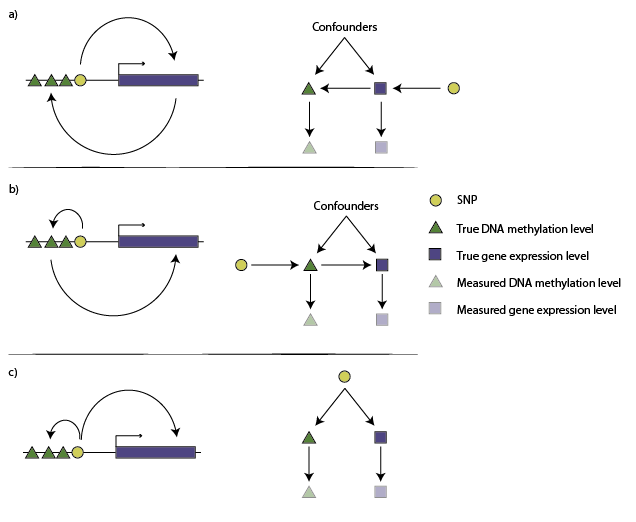
\includegraphics{../images/dag-01.png}

Figure 1: Gene expression levels (blue blocks) and DNA methylation
levels (green triangles) may be correlated but the causal structure is
unknown. If a SNP (yellow circle) is associated with both DNA
methylation and gene expression levels then it can be used as an
instrument, but there are three basic competing models for these
variables. The causal inference test (CIT) attempts to distinguish
between them. a) Methylation causes gene expression. The left figure
shows that the SNP influences methylation levels that in turn influence
gene expression levels. The right figure shows the directed acyclic
graph that represents this model. Faded symbols represent the measured
values whereas solid symbols represent the true values. b) The same as
in A, except the causal direction is from gene expression to DNA
methylation. c) A model of confounding, where gene expression and DNA
methylation are not causally related, but the SNP influences them each
through separate pathways or a confounder.

\newpage

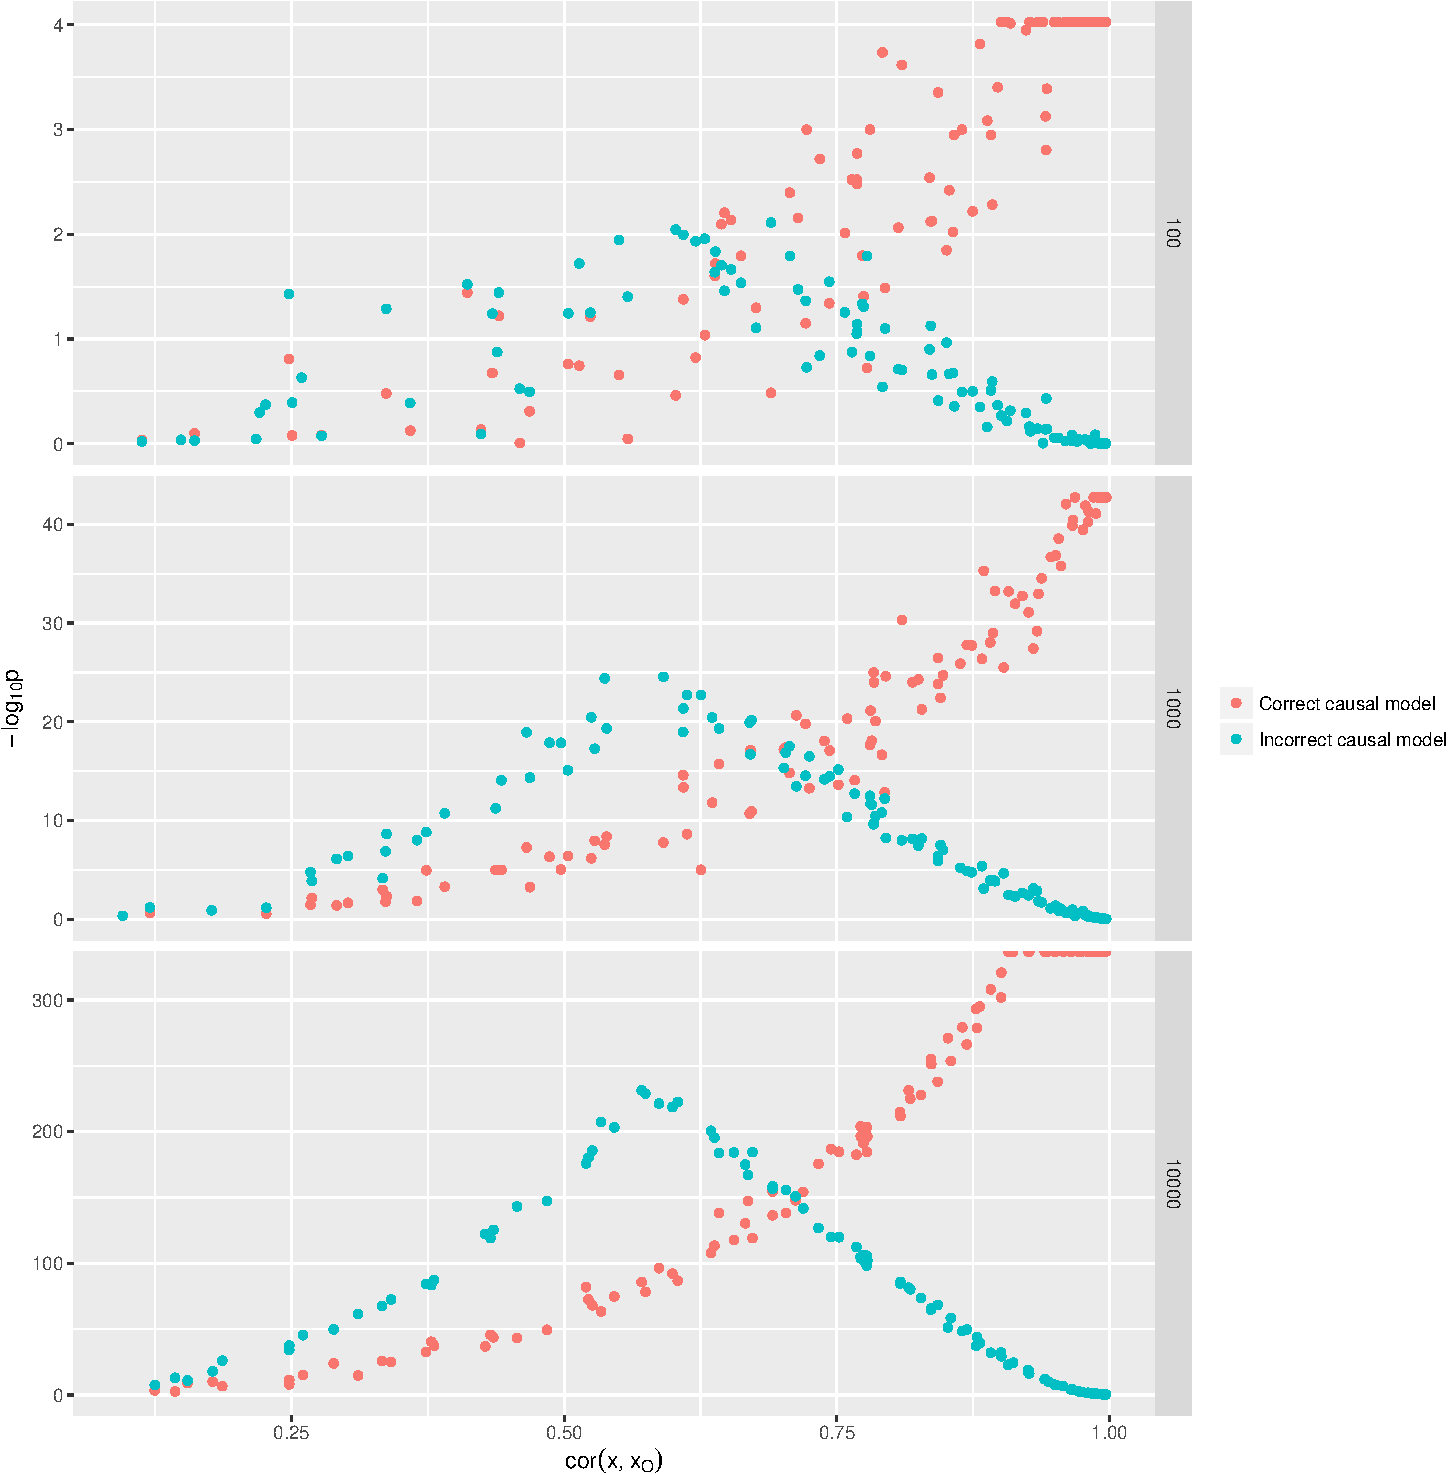
\includegraphics{manuscript_files/figure-latex/cit_measurement_error_figure-1.pdf}

Figure 2: The CIT was performed on simulated variables where the
exposure influenced the outcome and the exposure was instrumented by a
SNP. The test statistic from CIT when testing if the exposure caused the
outcome (the true model) is in red, and the test for the outcome causing
the exposure (false model) is in green. Rows of plots represent the
sample sizes used for the simulations. As measurement imprecision
increases (decreasing values on x-axis) the test statistic for the
incorrect model gets stronger and the test statistic for the correct
model gets weaker.

\newpage

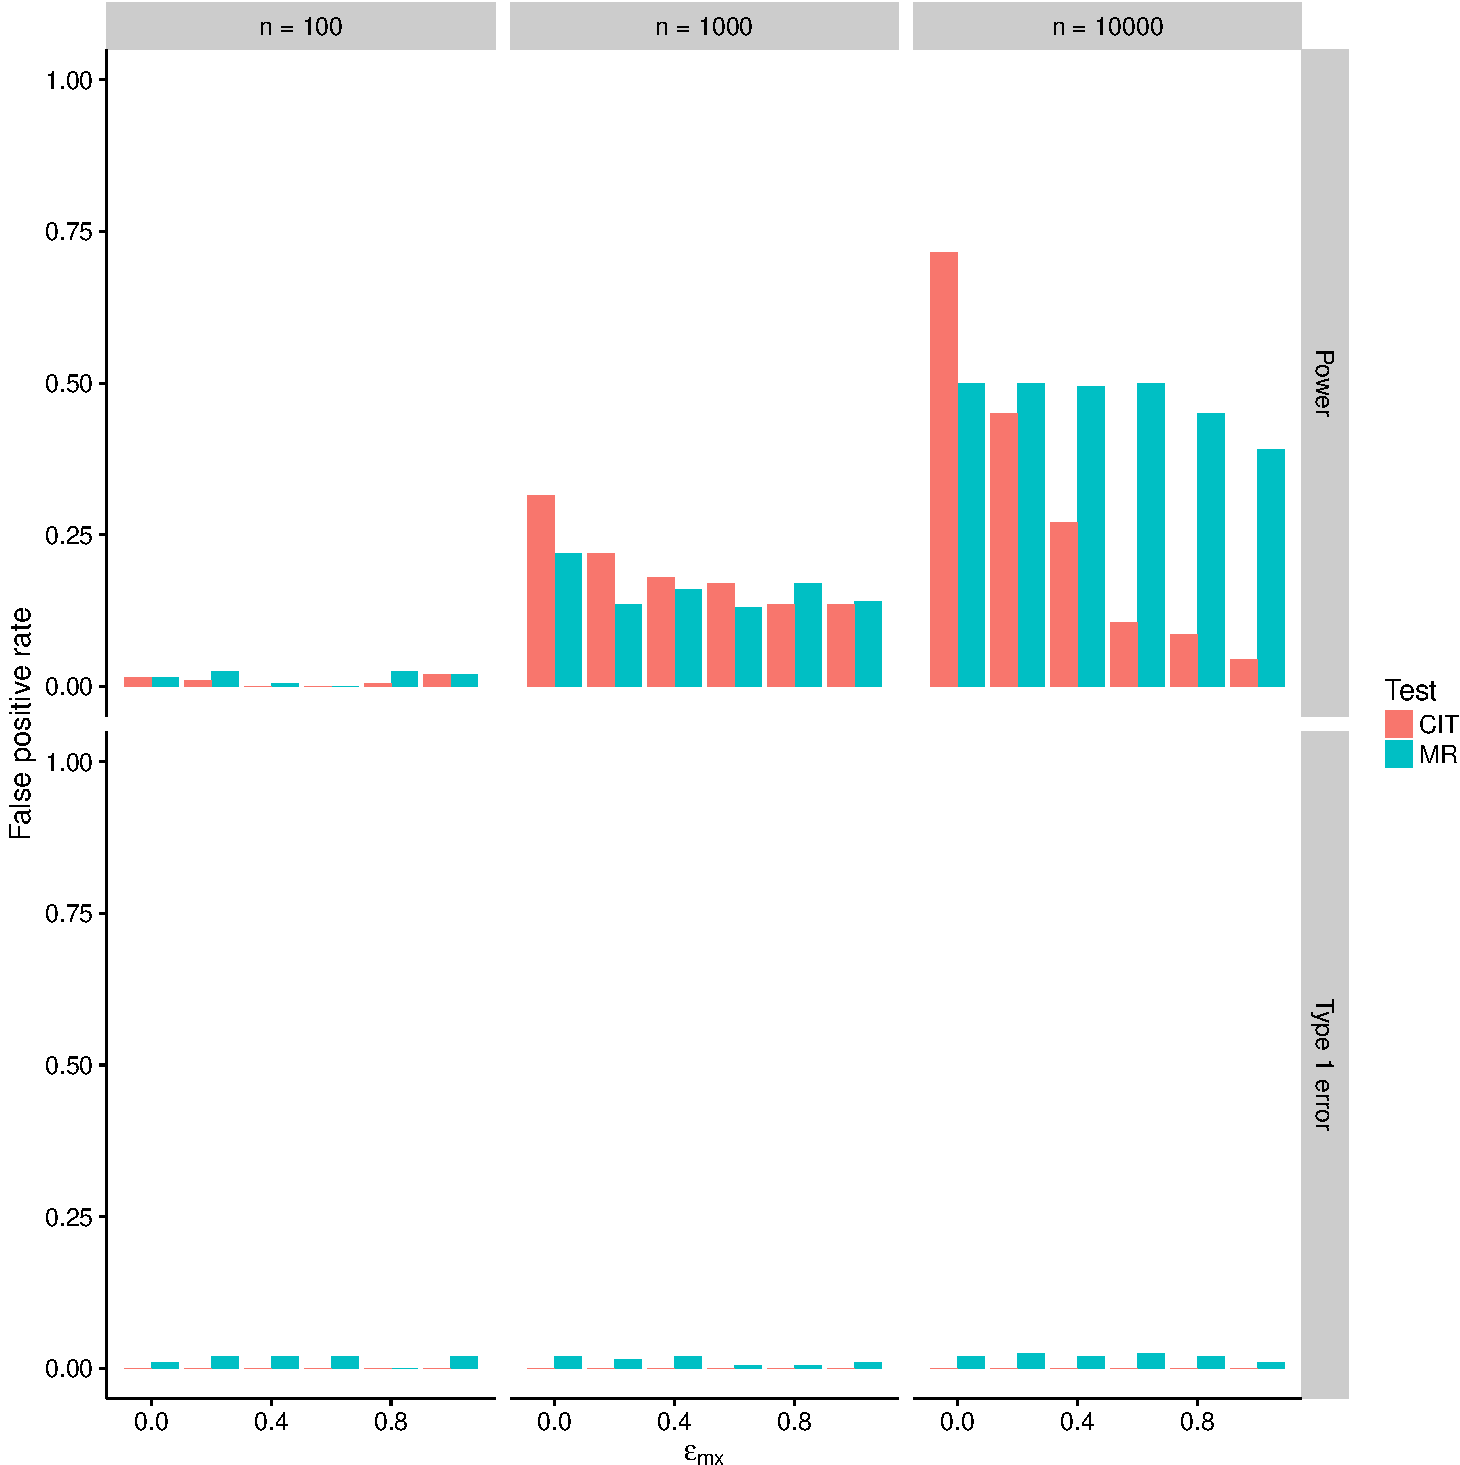
\includegraphics{manuscript_files/figure-latex/causality_exists_tpr-1.pdf}

Figure 3: Outcomes were simulated to be causally influenced by exposures
with varying degrees of measurement imprecision applied to the exposure
variable (x axis). True positive rates (y axis) for MR and CIT were
compared for varying levels of measurement imprecision in the outcome
variable (rows of boxes) and sample sizes (columns of boxes).

\newpage

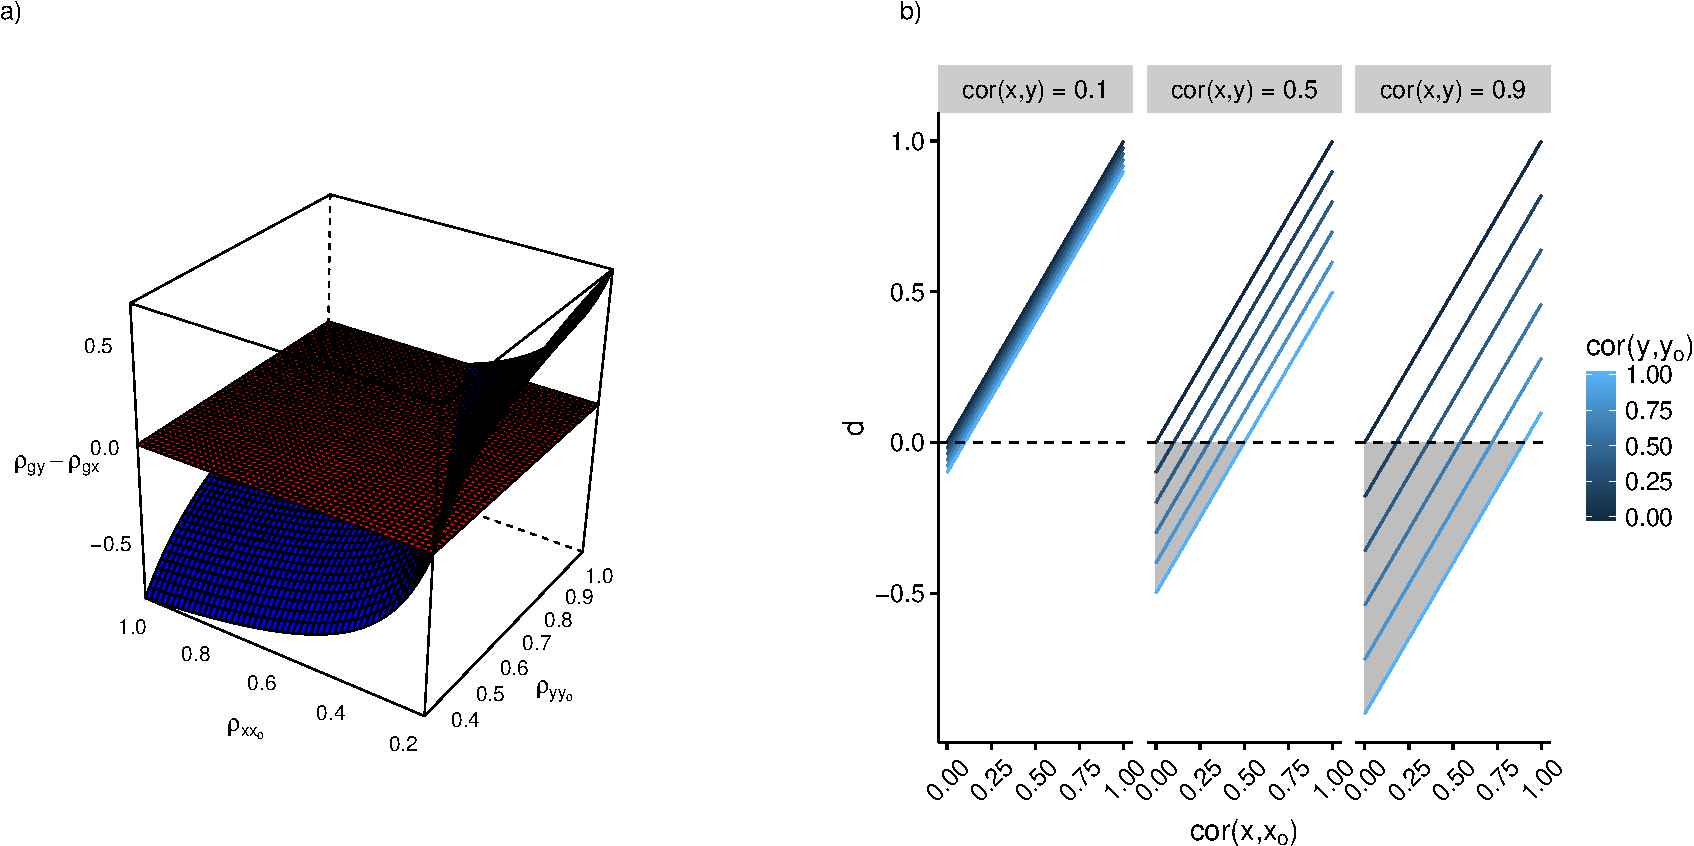
\includegraphics{manuscript_files/figure-latex/steiger_sensitivity_plot-1.pdf}

Figure 4: a) We can predict the values the Steiger test would take
(z-axis) for different potential values of measurement error (x and y
axes), drawn here as the blue surface. When \(\rho_{g,y} > \rho_{g,x}\),
as denoted by the range of values where the blue surface is above the
red plane, those values of measurement error lead to our observed
Steiger test inferring the wrong causal direction. Where the blue
surface lies below the red plane, these measurement error values support
the inferred causal direction of X to Y. A measure of reliability,
therefore, is the ratio of the negative and positive volumes of the
total space bound by the blue and red surfaces,
\(R = \frac{V_{z \geq 0}}{ - V_{z < 0} }\). In this case, where
\(\rho_{g,x}^2 = 0.01\) and \(\rho_{x,y}^2 = 0.1\), the \(R = 4.40\),
which means that 4.40 times as much of the possible measurement error
values are in support of the \(x \rightarrow y\) direction of causality
than \(y \rightarrow x\). b) Plots depicting the parameter space in
which the function \(d = cor(x, x_O) - cor(x,y)cor(y, y_O)\) is
negative. When \(d\) is negative the Steiger test is liable to infer the
wrong direction of causality. Shaded regions show the parameter space
where \(d\) is negative. The graph shows that for the majority of the
parameter space of the function, \(d\) is positive, especially where
causal relationships are relatively weak.

\newpage

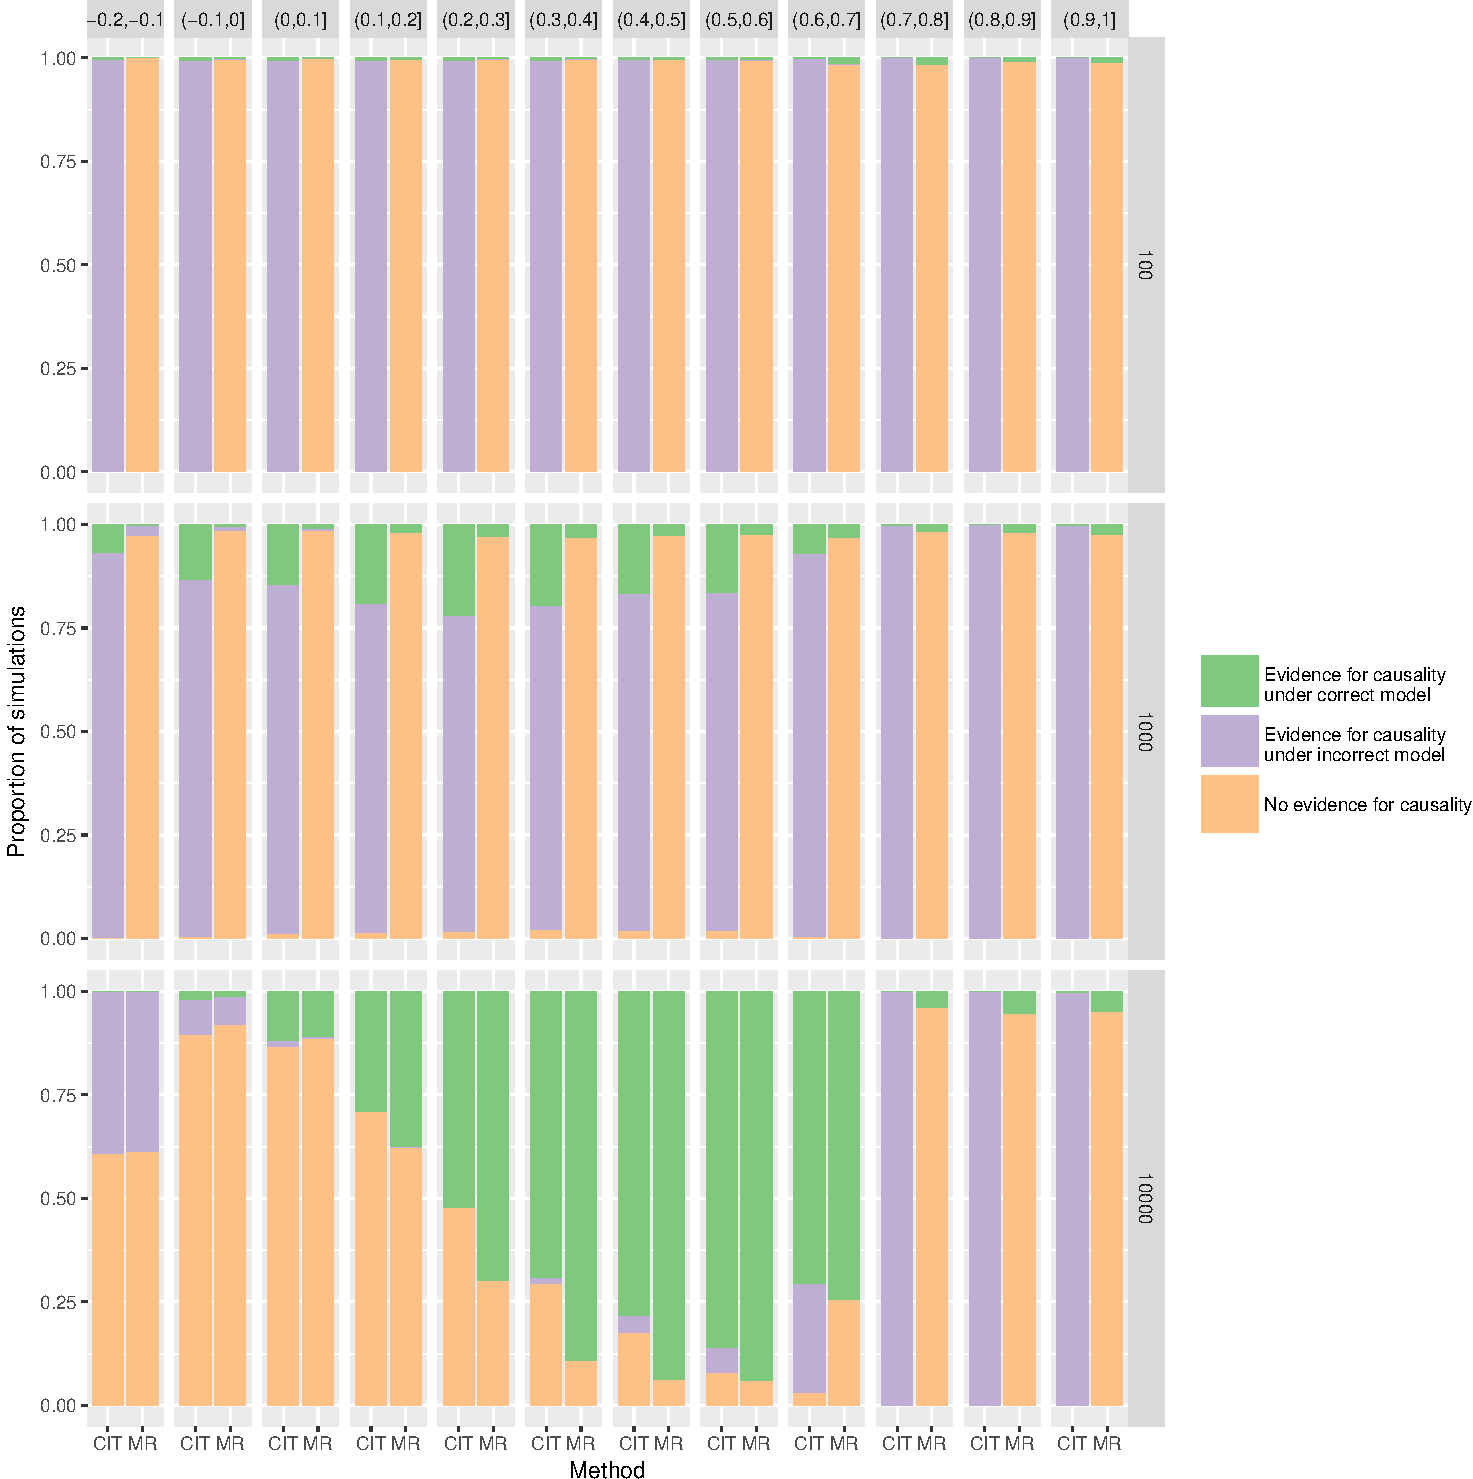
\includegraphics{manuscript_files/figure-latex/cit_mr_comparison_figure-1.pdf}

Figure 5: a) Outcome \(y\) was simulated to be caused by exposure \(x\)
as shown in the graph, with varying degrees of measurement error applied
to both. CIT and MR were used to infer evidence for causality between
the exposure and outcome, and to infer the direction of causality. The
value of \(d = \rho_{x, x_o} - \rho_{x,y}\rho_{y,y_o}\), such that when
\(d\) is negative we expect the Steiger test to be more likely to be
wrong about the direction of causality. Rows of graphs represent the
sample size used in the simulations. For the CIT method, outcome 1
denoted evidence for causality with correct model, outcomes 2 or 3
denoted evidence for causality with incorrect model, and outcome 4
denoted no evidence for causality. b) As in (a) except the simulated
model was non-causal, and a genetic confounder induces an association
between \(x\) and \(y\). MR is unable to identify this model, so any
significant associations are deemed to be incorrect. Outcome 3 denotes
evidence for the correct model for the CIT method.

\newpage

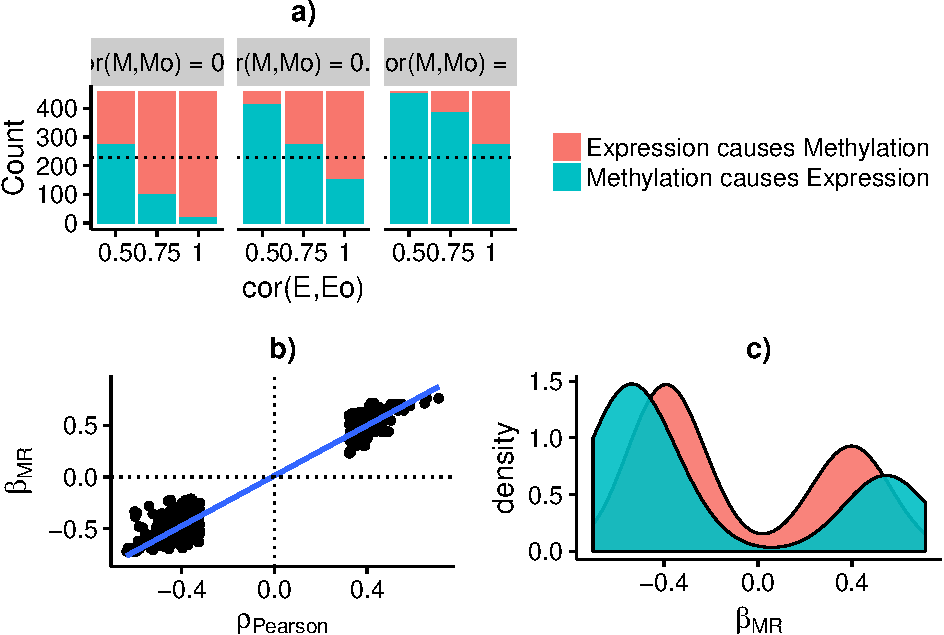
\includegraphics{manuscript_files/figure-latex/shakhplot-1.pdf}

Figure 6: Using 458 putative associations between DNA methylation and
gene expression we used the Steiger test to infer the direction of
causality between them. a) The rightmost bar shows the proportion of
associations for each of the two possible causal directions (colour key)
assuming no measurement error in either gene expression or DNA
methylation levels. The proportions change when we assume different
levels of measurement error in gene expression levels (x-axis) or DNA
methylation levels (columns of boxes). If there is systematically higher
measurement error in one platform than the other it will appear to be
less likely to be the causal factor. b) The relationship between the
Pearson correlation between DNA methylation and gene expression levels
(x-axis) and the causal estimate (scaled to be in standard deviation
units, y-axis). c) Distribution of estimated causal effect sizes,
stratified into associations inferred to be due to DNA methylation
causing expression (blue) and expression causing DNA methylation (red).

\newpage

\subsection{Appendix 1}\label{appendix-1}

We assume the following model

\[
\begin{aligned}
x   & = \alpha_g + \beta_g g + \epsilon_g \\
x_o & = \alpha_{mx} + \beta_{mx} x + \epsilon_{mx} \\
y   & = \alpha_x + \beta_x x + \epsilon_x \\
y_o & = \alpha_{my} + \beta_{my} y + \epsilon_{my}
\end{aligned}
\]

where \(x\) is the exposure on the outcome \(y\), \(g\) is an instrument
that has a direct effect on \(x\), \(x_o\) is the measured quantity of
\(x\), where measurement error is incurred from linear transformation in
\(\alpha_{mx}\) and \(\beta_{mx}\) and imprecision from
\(\epsilon_{mx}\), and \(y_o\) is the measured quantity of \(y\), where
measurement error is incurred from linear transformation in
\(\alpha_{my}\) and \(\beta_{my}\) and imprecision from
\(\epsilon_{my}\). Our objective is to estimate the expected magnitude
of association between \(g\) and \(y\) after conditioning on \(x\).
Under the CIT, this is expected to be \(cov(g, y_o - \hat{y}_o) = 0\)
when \(x\) causes \(y\), where
\(\hat{y}_o = \hat{a}_{x_o} + \hat{\beta}_{x_o} x_o\) is the predicted
value of \(y_o\) using the measured value of \(x_o\).

We can split \(cov(g, y_o - \hat{y}_o)\) into two parts, \(cov(g, y_o)\)
and \(cov(g, \hat{y}_o)\).

\textbf{Part 1}

\[
\begin{aligned}
cov(g, y_o) & = cov(g, \beta_{my} y) \\
            & = cov(g, \beta_{my} \beta_x x) \\
            & = cov(g, \beta_{my} \beta_x \beta_g g) \\
            & = \beta_{my} \beta_x \beta_g var(g)
\end{aligned}
\]

\textbf{Part 2}

\[
\begin{aligned}
cov(g, \hat{y}_o) & = cov(g, \hat{\beta}_{x_o} x_o) \\
                  & = cov(g, \hat{\beta}_{x_o} \beta_{mx} x) \\
                  & = cov(g, \hat{\beta}_{x_o} \beta_{mx} \beta_g g) \\
                  & = \hat{\beta}_{x_o} \beta_{mx} \beta_g var(g)
\end{aligned}
\]

Simpifying further

\[
\begin{aligned}
\hat{\beta}_{x_o} & = \frac{cov(y_o, x_o)} {var(x_o)} \\
                  & = \frac{cov(\beta_{my} y, \beta_{mx} x)} {\beta_{mx}^2 var(x) + var(\epsilon_{mx})} \\
                  & = \frac{\beta_{mx} \beta_{my} cov(y, x)} {\beta_{mx}^2 var(x) + var(\epsilon_{mx})} \\
                  & = \frac{\beta_{mx} \beta_{my} \beta_x var(x)} {\beta_{mx}^2 var(x) + var(\epsilon_{mx})}
\end{aligned}
\]

which can be substituted back to give

\[
\begin{aligned}
cov(g, \hat{y}_o) & = \frac{\beta_{my} \beta_x \beta_g var(g) \beta_{mx}^2 var(x)} {\beta_{mx}^2 var(x) + var(\epsilon_{mx})} \\
                  & = \frac{\beta_{mx}^2 var(x)} {\beta_{mx}^2 var(x) + var(\epsilon_{mx})} \times \beta_{my} \beta_x \beta_g var(g)
\end{aligned}
\]

Finally

\[
\begin{aligned}
cov(g, y_o - \hat{y}_o) & = \beta_{my} \beta_x \beta_g var(g) - \frac{\beta_{mx}^2 var(x)} {\beta_{mx}^2 var(x) + var(\epsilon_m)} \times \beta_{my} \beta_x \beta_g var(g)
\end{aligned}
\]

thus \(cov(g, y_o - \hat{y}_o) = 0\) if the measurement imprecision in
\(x_o\) is \(var(\epsilon_m) = 0\). However if there is any imprecision
then the condition \(cov(g, y_o - \hat{y}_o) = 0\) will not hold.

\subsection{Appendix 2}\label{appendix-2}

Assuming that either \(x \rightarrow y\) or \(y \rightarrow x\), the
causal direction can be inferred by evaluating which of \(\rho_{g, x}\)
and \(\rho_{g, y}\) is larger in magnitude. The Steiger test is a
hypothesis test that provides a p-value for observing the difference in
these correlations under the null hypothesis that they are equal.

Assuming the causal direction is \(x \to y\), two stage MR is formulated
using the following regression models:

\[
x = \alpha_1 + \beta_1 g + e_1
\]

for the first stage and

\[
y = \alpha_2 + \beta_2 \hat{x} + e_2
\]

where \(\hat{x} = \hat{\alpha}_1 + \hat{\beta}_1 g\). Writing in scale
free terms, \(\rho_{g, x}\) denotes the correlation between \(g\) and
the exposure variable \(x\), and it is expected that
\(\rho_{g, x} > \rho_{g, y}\) because
\(\rho_{g, y} = \rho_{g, x}\rho_{x, y}\), where \(\rho_{x, y}\) is the
causal association between \(x\) and \(y\) (which is likely to be less
than 1).

In the presence of measurement error in \(x\) and \(y\), however, the
empirical inference of the causal direction will instead be based on
evaluating \(\rho_{g, x_o} > \rho_{g, y_o}\), which can be simplified:

\[
\begin{aligned}
\rho_{g, x_O} & > \rho_{g, y_O} \\
\rho_{g, x} \rho_{x, x_O} & > \rho_{g,y}\rho_{y,y_O}\\
\rho_{g, x} \rho_{x, x_O} & > \rho_{g,x}\rho_{x,y}\rho_{y,y_O}\\
\rho_{x, x_O} & > \rho_{x,y}\rho_{y,y_O}
\end{aligned}
\]

In order to assess how reliable the inference of the causal direction is
in the presence of measurement imprecision, we can evaluate the range of
potential values of measurement error in \(x\) and \(y\) over which the
empirical difference in \(\rho_{g, x_o}\) and \(\rho_{g, y_o}\) would
return the wrong causal direction.

For different values of \(\rho_{x,x_o}\),
\(\rho_{g,x} = \frac{\rho_{g, x_o}}{\rho_{x,x_o}}\) and
\(\rho_{g,x_o} \leq \rho_{x,x_o} \leq 1\). For different values of
\(\rho_{y,y_o}\), \(\rho_{g,y} = \frac{\rho_{g, y_o}}{\rho_{y,y_o}}\)
and \(\rho_{g,y_o} \leq \rho_{y,x_o} \leq 1\).

Call \(z = \rho_{g,y} - \rho_{g,x}\) the true difference in the variance
explained by the genetic variant in \(y\) and \(x\). If \(z < 0\) then
we infer that \(x \rightarrow y\). There will be some values of
\(\rho_{x,x_o}\) and \(\rho_{y,y_o}\) that do not alter whether
\(z < 0\). To evaluate the reliability, \(R\), of the inference of the
causal direction with regards to measurement error, the objective is to
compare the proportion of the parameter space that agrees with the
inferred direction against the proportion which does not:

\[
R = \frac{V_{z \geq 0}}{ - V_{z < 0} }
\]

If \(R=1\) then the direction of causality is equally probable across
the range of possible measurement error values. If \(R > 1\) then \(R\)
times as much of the parameter space favours the inferred direction of
causality. \(V_{z}\), the total volume of the function (Figure 4), can
be obtained analytically by solving:

\[
\begin{aligned}
V_z & = \int^1_{\rho_{g,x_o}} \int^1_{\rho_{g,y_o}} \frac{\rho_{g,y_o}}{\rho_{y,y_o}} - \frac{\rho_{g,x_o}}{\rho_{x,x_o}}\,\,\,\, d\rho_{y,y_o}d\rho_{x,x_o} \\
& = \rho_{g,x_o}log(\rho_{g,x_o}) - \rho_{g,y_o}log(\rho_{g,y_o}) + \rho_{g,x_o}\rho_{g,y_o}(log(\rho_{g,y_o})-log(\rho_{g,x_o}))
\end{aligned}
\]

\(V_{z \ge 0}\), the proportion of the volume that lies above the
\(z=0\) plane, can also be obtained analytically. The region of this
volume is bound by the values of \(\rho_{x,x_o}\) and \(\rho_{y,y_o}\)
where \(0 = \rho_{g,y} - \rho_{g,x}\), which can be expanded to
\(\rho_{y,y_o} = \rho_{g,y_o}\rho_{x,x_o} / \rho_{g,x_o}\). Hence,

\[
\begin{aligned}
V_{z \ge 0} & = \int^1_{\rho_{g,x_o}} \int^{\frac{\rho_{g,y_o}\rho_{x,x_o}}{\rho_{g,x_o}}}_{\rho_{g,y_o}} \frac{\rho_{g,y_o}}{\rho_{y,y_o}} - \frac{\rho_{g,x_o}}{\rho_{x,x_o}}\,\,\,\, d\rho_{y,y_o}d\rho_{x,x_o} \\
& = 2\rho_{g,x_o}\rho_{g,y_o} - 2\rho_{g,y_o} - \rho_{g,y_o}log(\rho_{g,x_o}) - \rho_{g,x_o}\rho_{g,y_o}log(\rho_{g,x_o})
\end{aligned}
\]

Thus \(V_{z < 0} = V_{z} - V_{z \geq 0}\).

\newpage

\subsection*{References}\label{references}
\addcontentsline{toc}{subsection}{References}

\hypertarget{refs}{}
\hypertarget{ref-Phillips1991}{}
1. Phillips, A. N. \& Davey Smith, G. How independent are `independent'
effects? relative risk estimation when correlated exposures are measured
imprecisely. \emph{Journal of Clinical Epidemiology} \textbf{44,}
1223--1231 (1991).

\hypertarget{ref-DaveySmith2002}{}
2. Davey Smith, G. \& Ebrahim, S. Data dredging, bias, or confounding.
\emph{BMJ} \textbf{325,} (2002).

\hypertarget{ref-DaveySmith2004}{}
3. Davey Smith, G. \& Ebrahim, S. Mendelian randomization: prospects,
potentials, and limitations. \emph{International journal of
epidemiology} \textbf{33,} 30--42 (2004).

\hypertarget{ref-Millstein2009}{}
4. Millstein, J., Zhang, B., Zhu, J. \& Schadt, E. E. Disentangling
molecular relationships with a causal inference test. \emph{BMC
genetics} \textbf{10,} 23 (2009).

\hypertarget{ref-Aten2008}{}
5. Aten, J. E., Fuller, T. F., Lusis, A. J. \& Horvath, S. Using genetic
markers to orient the edges in quantitative trait networks: the NEO
software. \emph{BMC systems biology} \textbf{2,} 34 (2008).

\hypertarget{ref-Waszak2015}{}
6. Waszak, S. M. \emph{et al.} Variation and genetic control of
chromatin architecture in humans. \emph{Cell} \textbf{162,} 1039--1050
(2015).

\hypertarget{ref-Houle2011}{}
7. Houle, D., Pélabon, C., Wagner, G. \& Hansen, T. Measurement and
meaning in biology. \emph{The Quarterly Review of Biology} \textbf{86,}
3--34 (2011).

\hypertarget{ref-Hernan2009}{}
8. Hernán, M. a \& Cole, S. R. Invited Commentary: Causal diagrams and
measurement bias. \emph{American journal of epidemiology} \textbf{170,}
959--62; discussion 963--4 (2009).

\hypertarget{ref-Harper2013}{}
9. Harper, K. N., Peters, B. a \& Gamble, M. V. Batch effects and
pathway analysis: two potential perils in cancer studies involving DNA
methylation array analysis. \emph{Cancer epidemiology, biomarkers \&
prevention : a publication of the American Association for Cancer
Research, cosponsored by the American Society of Preventive Oncology}
\textbf{22,} 1052--60 (2013).

\hypertarget{ref-Chen2013a}{}
10. Chen, Y.-a. \emph{et al.} Discovery of cross-reactive probes and
polymorphic CpGs in the Illumina Infinium HumanMethylation450
microarray. \emph{Epigenetics : official journal of the DNA Methylation
Society} \textbf{8,} 203--9 (2013).

\hypertarget{ref-Houseman2012}{}
11. Houseman, E. A. \emph{et al.} DNA methylation arrays as surrogate
measures of cell mixture distribution. \emph{BMC bioinformatics}
\textbf{13,} 86 (2012).

\hypertarget{ref-Ahima2013}{}
12. Ahima, R. S. \& Lazar, M. A. Physiology. The health risk of
obesity--better metrics imperative. \emph{Science (New York, N.Y.)}
\textbf{341,} 856--8 (2013).

\hypertarget{ref-LeCessie2012}{}
13. Cessie, S. le, Debeij, J., Rosendaal, F. R., Cannegieter, S. C. \&
Vandenbroucke, J. P. Quantification of bias in direct effects estimates
due to different types of measurement error in the mediator.
\emph{Epidemiology (Cambridge, Mass.)} \textbf{23,} 551--60 (2012).

\hypertarget{ref-Blakely2013}{}
14. Blakely, T., McKenzie, S. \& Carter, K. Misclassification of the
mediator matters when estimating indirect effects. \emph{Journal of
epidemiology and community health} \textbf{67,} 458--66 (2013).

\hypertarget{ref-DaveySmith2003}{}
15. Davey Smith, G. \& Ebrahim, S. 'Mendelian randomization': can
genetic epidemiology contribute to understanding environmental
determinants of disease? \emph{International Journal of Epidemiology}
\textbf{32,} 1--22 (2003).

\hypertarget{ref-DaveySmithHemani2014}{}
16. Davey Smith, G. \& Hemani, G. Mendelian randomization: genetic
anchors for causal inference in epidemiological studies. \emph{Human
molecular genetics} \textbf{23,} R89-----R98 (2014).

\hypertarget{ref-Schadt2005}{}
17. Schadt, E. E. \emph{et al.} An integrative genomics approach to
infer causal associations between gene expression and disease.
\emph{Nature Genetics} \textbf{37,} 710--717 (2005).

\hypertarget{ref-Millstein2016}{}
18. Millstein, J., Chen, G. K. \& Breton, C. V. Cit : Hypothesis Testing
Software for Mediation Analysis in Genomic Applications.
\emph{Bioinformatics} \textbf{AOP,} 1--10 (2016).

\hypertarget{ref-Koestler2014}{}
19. Koestler, D. C. \emph{et al.} Integrative genomic analysis
identifies epigenetic marks that mediate genetic risk for epithelial
ovarian cancer. \emph{BMC medical genomics} \textbf{7,} 8 (2014).

\hypertarget{ref-Liu2013}{}
20. Liu, Y. \emph{et al.} Epigenome-wide association data implicate DNA
methylation as an intermediary of genetic risk in rheumatoid arthritis.
\emph{Nature biotechnology} \textbf{31,} 142--7 (2013).

\hypertarget{ref-Yuan2014}{}
21. Yuan, W. \emph{et al.} An integrated epigenomic analysis for type 2
diabetes susceptibility loci in monozygotic twins. \emph{Nature
communications} \textbf{5,} 5719 (2014).

\hypertarget{ref-Tang2014}{}
22. Tang, Y. \emph{et al.} Genotype-based treatment of type 2 diabetes
with an \(\alpha\)2A-adrenergic receptor antagonist. \emph{Science
translational medicine} \textbf{6,} 257ra139 (2014).

\hypertarget{ref-Hong2015}{}
23. Hong, X. \emph{et al.} Genome-wide association study identifies
peanut allergy-specific loci and evidence of epigenetic mediation in US
children. \emph{Nature communications} \textbf{6,} 6304 (2015).

\hypertarget{ref-Bowden2015}{}
24. Bowden, J., Davey Smith, G. \& Burgess, S. Mendelian randomization
with invalid instruments: effect estimation and bias detection through
Egger regression. \emph{International Journal of Epidemiology}
\textbf{In press,} (2015).

\hypertarget{ref-Bowden2016b}{}
25. Bowden, J., Davey Smith, G., Haycock, P. C. \& Burgess, S.
Consistent Estimation in Mendelian Randomization with Some Invalid
Instruments Using a Weighted Median Estimator. \emph{Genetic
Epidemiology} \textbf{40,} 304--314 (2016).

\hypertarget{ref-Hemani2016}{}
26. Hemani, G. \emph{et al.} MR-Base: a platform for systematic causal
inference across the phenome using billions of genetic associations.
\emph{BioRxiv} \textbf{10.1101/07,} (2016).

\hypertarget{ref-Claussnitzer2015}{}
27. Claussnitzer, M. \emph{et al.} FTO Obesity Variant Circuitry and
Adipocyte Browning in Humans. \emph{The New England journal of medicine}
\textbf{373,} 895--907 (2015).

\hypertarget{ref-Pierce2013}{}
28. Pierce, B. L. \& Burgess, S. Efficient design for Mendelian
randomization studies: subsample and 2-sample instrumental variable
estimators. \emph{American journal of epidemiology} \textbf{178,}
1177--84 (2013).

\hypertarget{ref-Pierce2012}{}
29. Pierce, B. L. \& VanderWeele, T. J. The effect of non-differential
measurement error on bias, precision and power in Mendelian
randomization studies. \emph{International Journal of Epidemiology}
\textbf{41,} 1383--1393 (2012).

\hypertarget{ref-Ashenfelter1994}{}
30. Ashenfelter, O. \& Krueger, A. B. Estimates of the Economic Return
to Schooling from a New Sample of Twins. \emph{The American Economic
Review} \textbf{84,} 1157--1173 (1994).

\hypertarget{ref-Nagarajan2013}{}
31. Nagarajan, R. \& Scutari, M. Impact of noise on molecular network
inference. \emph{PloS one} \textbf{8,} e80735 (2013).

\hypertarget{ref-Shpitser2010}{}
32. Shpitser, I., VanderWeele, T. \& Robins, J. On the validity of
covariate adjustment for estimating causal effects. \emph{Proceedings of
the Twenty Sixth Conference on Uncertainty in Artificial Intelligence
(UAI-10)} 527--536 (2010).

\hypertarget{ref-Wang2015}{}
33. Wang, L. \& Michoel, T. Detection of regulator genes and eQTLs in
gene networks. \emph{arXiv} \textbf{arXiv:1512,} (2015).

\hypertarget{ref-Lagani2015}{}
34. Lagani, V., Triantafillou, S., Ball, G., Tegner, J. \& Tsamardinos,
I. in \emph{Uncertainty in biology: A computational modeling approach}
47 (Springer, 2015). at
\textless{}\href{https://books.google.com/books?id=8SLUCgAAQBAJ\%7B/\&\%7Dpgis=1}{https://books.google.com/books?id=8SLUCgAAQBAJ\{\textbackslash{}\&\}pgis=1}\textgreater{}

\hypertarget{ref-Lawlor2017}{}
35. Lawlor, D. A., Tilling, K. \& Davey Smith, G. Triangulation in
aetiological epidemiology. \emph{International Journal of Epidemiology}
\textbf{19,} dyw314 (2017).

\hypertarget{ref-Sterne2001}{}
36. Sterne, J. A. C., Cox, D. R. \& Smith, G. D. Sifting the
evidence---what's wrong with significance tests?Another comment on the
role of statistical methods. \emph{BMJ} \textbf{322,} (2001).

\hypertarget{ref-Henningsen2007}{}
37. Henningsen, A. \& Hamann, J. D. systemfit : A Package for Estimating
Systems of Simultaneous Equations in R. \emph{Journal of Statistical
Software} \textbf{23,} 1--40 (2007).

\hypertarget{ref-Steiger1980}{}
38. Steiger, J. H. Tests for comparing elements of a correlation matrix.
\emph{Psychological Bulletin} \textbf{87,} 245--251 (1980).

\hypertarget{ref-Revelle2015}{}
39. Revelle, W. \emph{psych: Procedures for Psychological, Psychometric,
and Personality Research}. (Northwestern University, 2015). at
\textless{}\url{http://cran.r-project.org/package=psych}\textgreater{}

\hypertarget{ref-Shakhbazov2016}{}
40. Shakhbazov, K. \emph{et al.} Shared genetic control of expression
and methylation in peripheral blood. \emph{BMC genomics} \textbf{17,}
278 (2016).

\hypertarget{ref-RCoreTeam2015}{}
41. R Core Team. \emph{R: A Language and Environment for Statistical
Computing}. (R Foundation for Statistical Computing, 2015). at
\textless{}\url{https://www.r-project.org/}\textgreater{}

\hypertarget{ref-Bird2002}{}
42. Bird, A. DNA methylation patterns and epigenetic memory. \emph{Genes
\& development} \textbf{16,} 6--21 (2002).

\hypertarget{ref-Cole2014}{}
43. Cole, D. A. \& Preacher, K. J. Manifest Variable Path Analysis:
Potentially Serious and Misleading Consequences Due to Uncorrected
Measurement Error. \emph{Psychological Methods} \textbf{19,} 300--315
(2014).

\hypertarget{ref-Bose2014}{}
44. Bose, M. \emph{et al.} Evaluation of microarray-based DNA
methylation measurement using technical replicates: the Atherosclerosis
Risk In Communities (ARIC) Study. \emph{BMC Bioinformatics} \textbf{15,}
312 (2014).

\hypertarget{ref-Bryant2011}{}
45. Bryant, P. A. \emph{et al.} Technical Variability Is Greater than
Biological Variability in a Microarray Experiment but Both Are
Outweighed by Changes Induced by Stimulation. \emph{PLoS ONE}
\textbf{6,} e19556 (2011).

\hypertarget{ref-Richmond2014}{}
46. Richmond, R. C. \emph{et al.} Assessing Causality in the Association
between Child Adiposity and Physical Activity Levels: A Mendelian
Randomization Analysis. \emph{PLoS Medicine} \textbf{11,} e1001618
(2014).

\hypertarget{ref-Lee2013c}{}
47. Lee, S. H. \& Wray, N. R. Novel genetic analysis for case-control
genome-wide association studies: quantification of power and genomic
prediction accuracy. \emph{PLoS One} \textbf{8,} e71494 (2013).

\hypertarget{ref-Relton2012}{}
48. Relton, C. L. \& Davey Smith, G. Two-step epigenetic Mendelian
randomization: a strategy for establishing the causal role of epigenetic
processes in pathways to disease. \emph{International journal of
epidemiology} \textbf{41,} 161--76 (2012).

\hypertarget{ref-Burgess2014a}{}
49. Burgess, S., Freitag, D. F., Khan, H., Gorman, D. N. \& Thompson, S.
G. Using multivariable Mendelian randomization to disentangle the causal
effects of lipid fractions. \emph{PloS one} \textbf{9,} e108891 (2014).

\hypertarget{ref-Varbo2015}{}
50. Varbo, A. \emph{et al.} Remnant cholesterol, low-density lipoprotein
cholesterol, and blood pressure as mediators from obesity to ischemic
heart disease. \emph{Circulation research} \textbf{116,} 665--73 (2015).

\hypertarget{ref-Burgess2015}{}
51. Burgess, S., Daniel, R. M., Butterworth, A. S. \& Thompson, S. G.
Network Mendelian randomization: using genetic variants as instrumental
variables to investigate mediation in causal pathways.
\emph{International journal of epidemiology} \textbf{44,} 484--95
(2015).

\hypertarget{ref-Richmond2016}{}
52. Richmond, R. C., Hemani, G., Tilling, K., Davey Smith, G. \& Relton,
C. L. Challenges and novel approaches for investigating molecular
mediation. \emph{Human molecular genetics} \textbf{25,} R149--R156
(2016).


\end{document}
